\documentclass[12pt, border = 4pt, multi]{article} % \documentclass[tikz, border = 4pt, multi]{article}
\usepackage[a4paper, margin = 70pt]{geometry}
\usepackage{lingmacros}
\usepackage{tree-dvips}
\usepackage{amssymb} % mathbb{}
\usepackage[dvipsnames]{xcolor}
\usepackage{forest}
\usepackage[pdftex]{hyperref}
\usepackage{amsmath} % matrices
\usepackage{xeCJK}
\usepackage{tikz}
\usepackage[arrowdel]{physics}
\usepackage{graphicx}
\usepackage{wrapfig}
\usepackage{listings}
\usepackage{pgfplots, pgfplotstable}
\usepackage{diagbox} % diagonal line in cell
\usepackage[usestackEOL]{stackengine}
\usepackage{makecell}
\usepackage{multirow}
\usepackage{multicol}
\usepackage[T1]{fontenc} 
\setlength{\columnsep}{1cm}
\graphicspath{{./img}} % specify the graphics path to be relative to the main .tex file, denoting the main .tex file directory as ./
\definecolor{orchid}{rgb}{0.7, 0.4, 1.1}
\lstset
{ 
  backgroundcolor = \color{white},
  basicstyle = \scriptsize,
  breaklines = true,
  commentstyle = \color{comment_color}\textit,
  keywordstyle = \color{keyword_color}\bfseries,
  language = c++,
  escapeinside = {\%*}{*)},          
  extendedchars = true,              
  frame = tb,
  numberstyle = \tiny\color{comment_color},
  rulecolor = \color{black},
  showstringspaces = false,
  stringstyle = \color{string_color},
  upquote = true, 
}
\usepackage{xcolor}
\definecolor{comment_color}{rgb}{0, 0.5, 0}
\definecolor{keyword_color}{rgb}{0.3, 0, 0.6}
\definecolor{string_color}{rgb}{0.5, 0, 0.1}
\begin{document}
\section*{Xi Liu}
last name: Liu\\
first name: Xi\\
netid: xl3504\\
\begin{verbatim}
• You may use the textbook, slides, and any notes you have.
But you may not use the internet.
• You may NOT use communication tools to collaborate 
with other humans. This includes but is not limited to
Google-Chat, Messenger, E-mail, etc.
• Do not try to search for answers on the internet
it will show in your answer, and you will earn an immediate grade of 0.
• Anyone found sharing answers or communicating
with another student during the exam
period will earn an immediate grade of 0.
• “I understand the ground rules and agree to abide by them.
I will not share answers or assist another student during this exam,
nor will I seek assistance from another student or attempt to view their answers.”
\end{verbatim}
\newpage
\noindent
Problem 1\\
a\\
advantage 1: no runtime dependencies since libraries are already linked at compile time\\
advantage 2: easier to manage, since contents of static libraries are copied to executable files that have symbol reference to the static libraries, may perform faster if the program have frequent use of library functions\\
\\
b\\
disadvantage 1: can take more space than dynamic linking, commonly used functions in stdio.h or stdlib.h can be replicated in each process's address space if the program uses the functions\\
disadvantage 2: if a programmer want to use newer version of a library, need to manually relink program to new version of the library, so is harder to maintain\\
\\
c\\
advantage 1: can take less space than static linking, required functions are linked at runtime when the program uses the functions\\
advantage 2: do not need to manually relink to use updated functions in shared libraries\\
\\
d\\
disadvantage 1: can have runtime dependencies since the shared object file need to be usable at runtime to execute the binary file\\
disadvantage 2: may take more time than static linking, for example, a page fault may happen if the pages containing shared library file is not found in main memory\\
\\
e\\
yes, after clicking an icon or typing a command, it might call fork() and execve(), required functions can be dynamically linked using dlopen() and dlsym() and then called. during the execution of the application, the application can use the dynamic linker to load and link shared libraries containing the functions to be used\\
\\
f\\
case 1:\\
if assume there is no printf("End of program\verb|\n|") inside the program with the name progname1 or progname2\\
then "End of program" will be printed 0 times. since after execve(progname1), the program with the name progname1 will be run\\
\\
case 2: (since the contents of progname1 is not explicitly given)\\
$\forall n \in \mathbb{N}$, if there are $n$ printf("End of program\verb|\n|") statements inside the program with the name progname1 and assuming there is no other additional execve() for the rest of the code,\\
then "End of program" will be printed $n$ times. since after execve(progname1), the program with the name progname1 will be run\\
\newpage
\noindent
Problem 2\\
following dependencies can be seen: 0 after 3. 0 after 2. 0 before 4. 0 after 4. 0 should be seen before 4 since the child process need to terminate for a state change and then wait() returns\\
\\
a
\begin{figure}[h!]
	\centering
	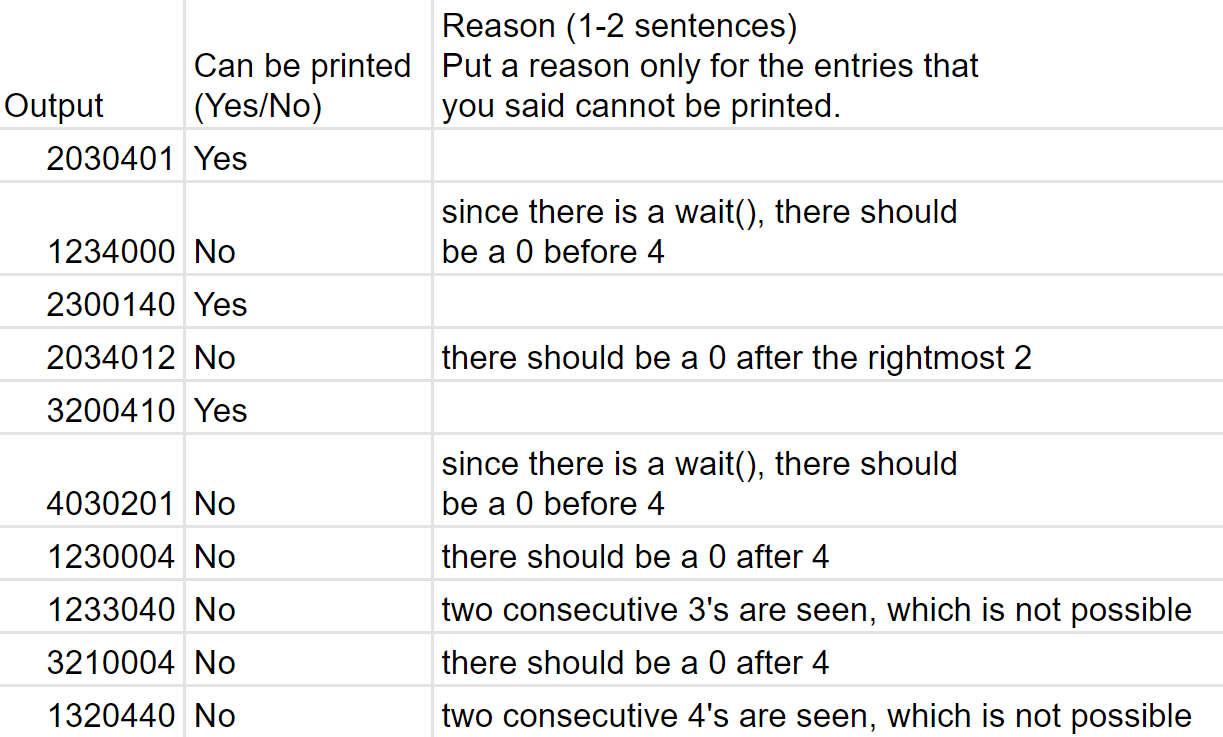
\includegraphics[width = 1.1\textwidth, height = 0.7\textwidth]{2} %img size
\end{figure}\\
\\
\\
b\\
4 processes are created in total\\
\\
\\
c\\
3 processes executed the line "return 0". since there is 1 process that called exit(0), upon execution of exit(0), the process would terminate and not return. so there are 4 - 1 = 3 processes that returned\\
\newpage
\noindent
Problem 3
\begin{figure}[h!]
	\centering
	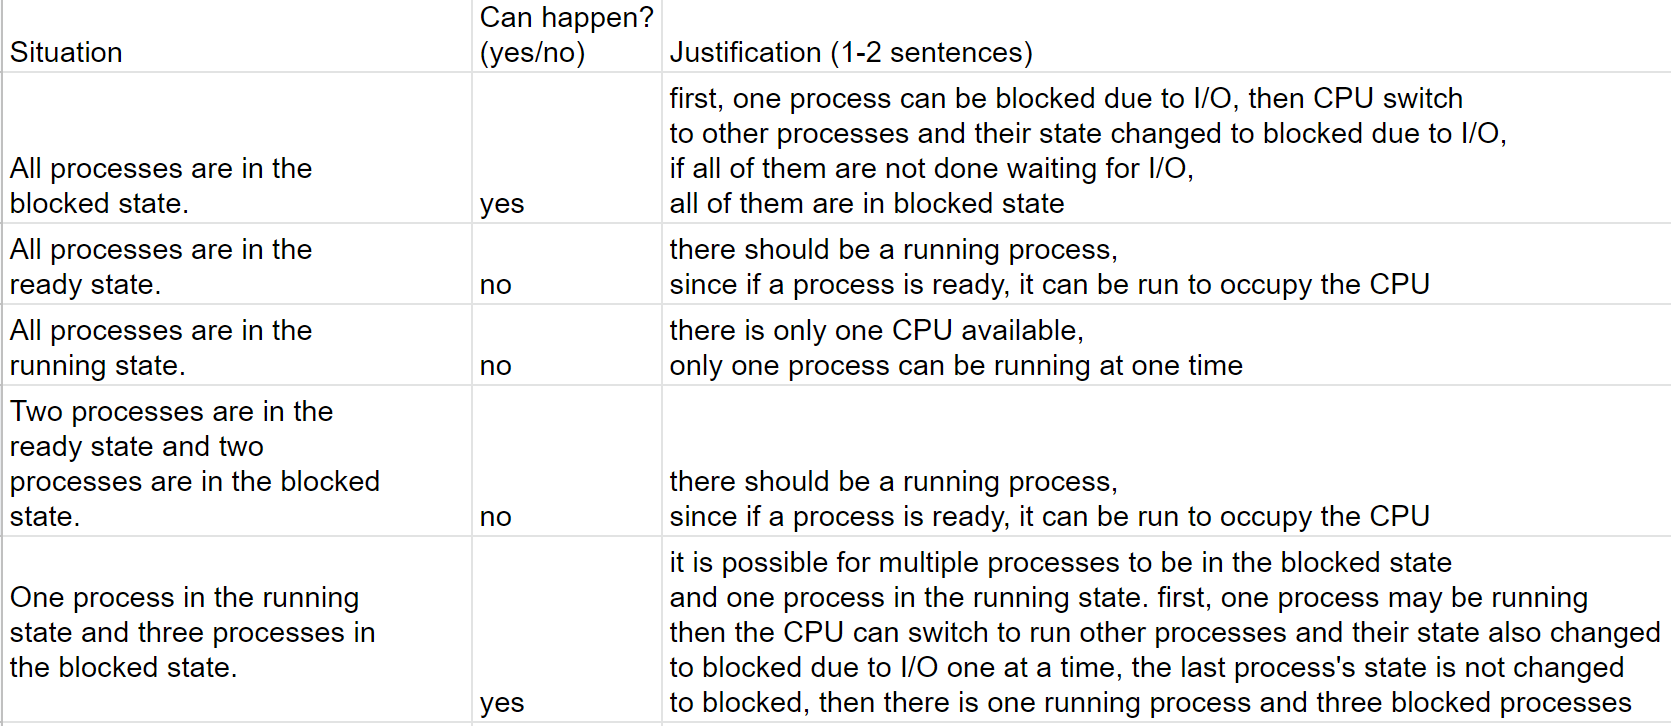
\includegraphics[width = 1.1\textwidth, height = 0.7\textwidth]{3} %img size
\end{figure}\\
\newpage
\noindent
Problem 4\\
a\\
yes, for example, if A caused some access violation, fault such as segmentation fault, or calls sleep() before it finishes its whole execution, then the CPU can run other processes (B, C, D) instead\\
\\
b\\
1. after a process have ran for a time slice or scheduling quantum, CPU switches to run another process\\
2. input/output (I/O), a process is removed from the CPU if it changes from running to blocked\\
3. when a process completes all that it needs to do, it exits or terminates normally, then it is removed from CPU\\
4. if the running process caused some irreversible hardware error or fault caused by some invalid operation, the process is likely to be removed from CPU\\
5. after exec(), the current process image (stack, heap, data segments, ...) is replaced with a new process image\\
\\
c\\
1. preemptive\\
2. false\\
3. false\\
4. false\\
5. true
\end{document}